\begin{frame}{CDMX Covid-19 data}
	%
	\begin{textblock*}{120mm}(3mm, 20mm)
		\only<1->{
			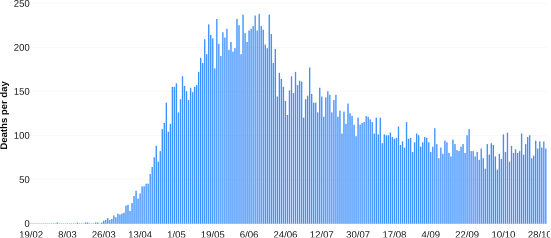
\includegraphics[width=\textwidth, keepaspectratio]{%
						assets/cdmx_dta.png
			}
		}	
	\end{textblock*}	
	%
	\begin{textblock*}{120mm}(70mm, 20mm)
		\only<2>{
			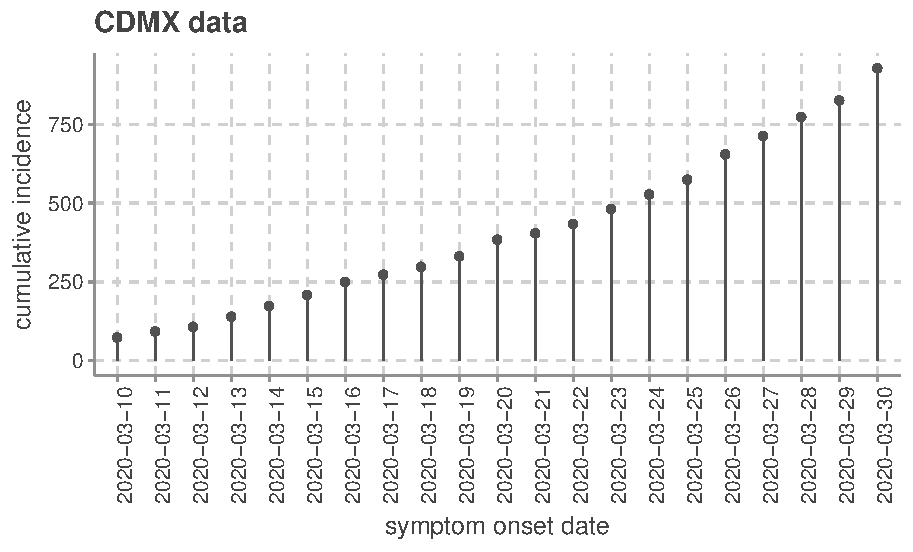
\includegraphics[width=0.4\textwidth, keepaspectratio]{%
				assets/cdmx_input_data}
		}
	\end{textblock*}
\end{frame}
%------------------------------------------------------------


\begin{frame}{First attempt: MCMC with a deterministic SEIRS structure}

	\begin{textblock*}{120mm}(0mm, 10mm)
		\only<1->{        
			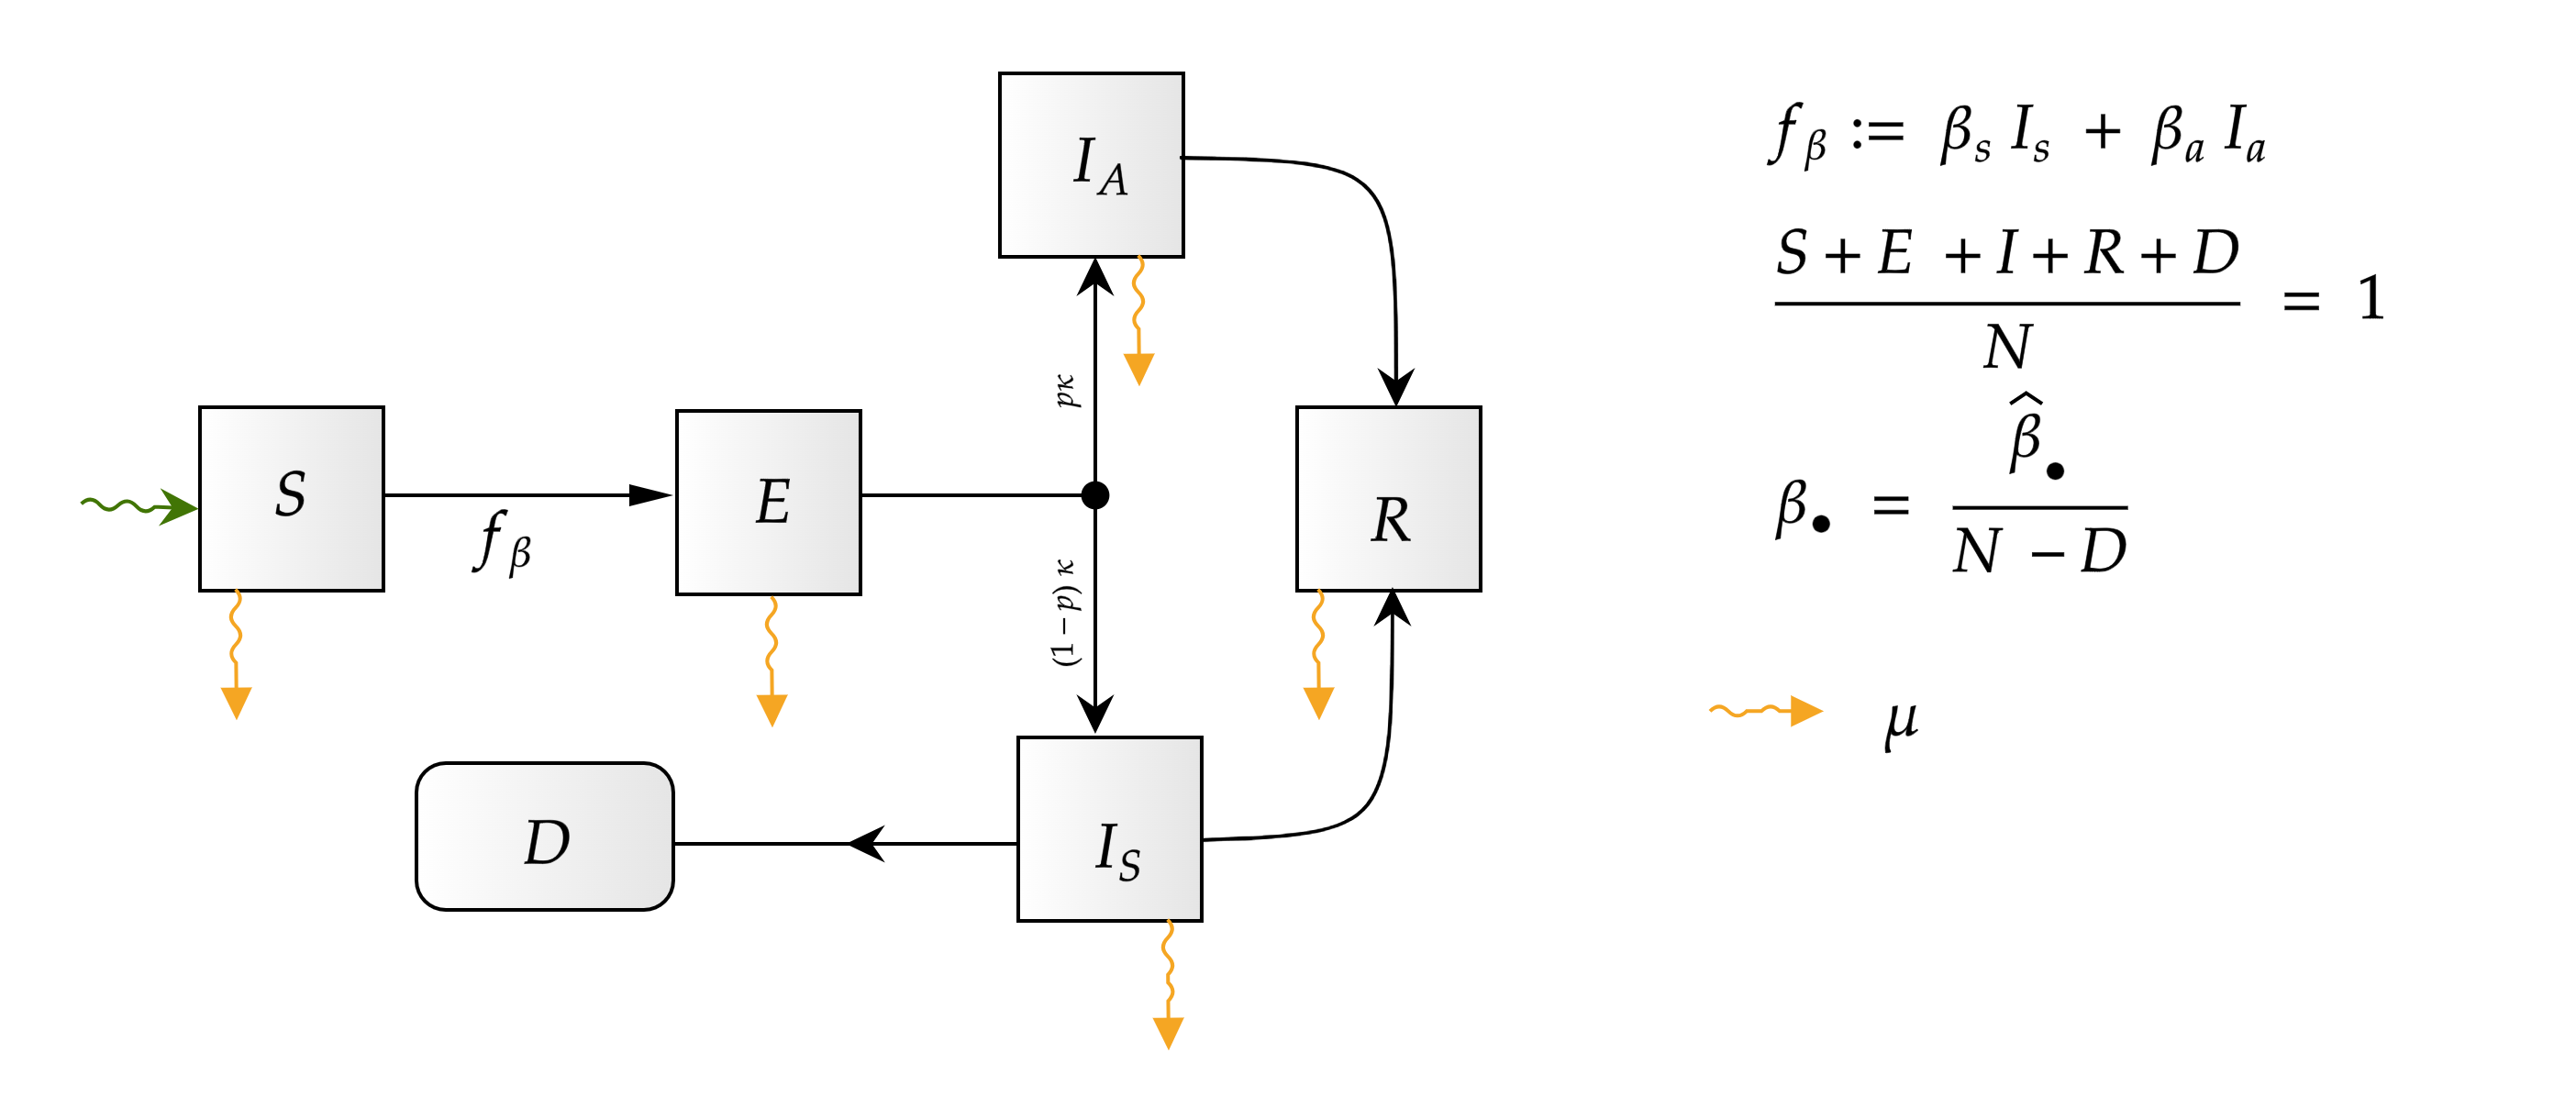
\includegraphics[width=\textwidth]{assets/stoSEIR_diagram.png} 
		}
	\end{textblock*}    
%    
%%    
	\begin{textblock*}{60mm}(0mm, 50mm)
		\only<2->{
			\begin{equation*}
				\label{eqn:base_dynamics}
				\begin{aligned}
					S'  &=
						\mu +\gamma R
						- \left(\mu  + f_{\beta} \right)  S
					\\
					E' & =  f_{\beta}S
						- (\kappa E + \mu E)
					\\
					{I_a}' &=
						p \kappa E
						- \big(\alpha_a + \mu \big)I_a
					\\
					{I_s}' &=
						(1 - p) \kappa E
						- (\alpha_s +\mu)  I_s
					\\
					{R}' &=
						\alpha_a I_a + \alpha_s (1 - \theta)I_s -
						(\mu + \gamma) R
					\\
					D' &= \theta \alpha_s I_s.
				\end{aligned}
			\end{equation*}
		}
	\end{textblock*}
	\begin{textblock*}{60mm}(67mm, 43mm)
		\only<3->{
			$$
				\mathcal{R}_0^{D}:=
					\dfrac{p \kappa \beta_s }{(\mu + \kappa) (\mu + \alpha_s)}
					+
					\dfrac{(1 - p) \kappa \beta_a}{(\mu + \kappa)(\mu + \alpha_a)}.
			$$
		}
	\end{textblock*}
%%    
	\begin{textblock*}{60mm}(65mm, 55mm)
		\only<3>{
			\begin{equation*}
				\label{eqn:base_dynamics_counter}
				\begin{aligned}
					Y_t & \sim
					\mathrm{Poisson}(\lambda_t)
					\\
					\lambda_t =& \int_0 ^ t (1-p) \kappa E
					\\
					p & \sim
					\mathrm{Uniform}(0.3, 0.8)
					\\
					\kappa & \sim
					\mathrm{Gamma}(10, 50)
					\\
					\beta_a, \beta_s & \sim \mathcal{N}(0.5, 0.1)    
			\end{aligned}
		\end{equation*}
		}
	\end{textblock*}
\end{frame}
%-------------------------------------------------------------------
\begin{bibunit}[plain]
	\begin{frame}{Parameter values of the deterministic model} %
	   \begin{textblock*}{120mm}(5mm,10mm)
		   \begin{table}
			\centering
			\begin{tabular}{ccc}
				\hline
				Parameter & Value & Reference\\ 
					\hline
				$\mu^{-1}$ & $70 \times 365$ & \cite{Acunya2021} 
				\\
				$\beta_s$ & 0.05821 & Estimated
				\\
				$\beta_a$ & 0.510968 & Estimated\\
				$\kappa$ & $0.196078^{-1}$ &  \cite{Tian2020}
				\\
				$p$ & 0.585505& Estimated\\          
				$\theta$ & 0.11 & \cite{Acunya2021}
				\\
				$\alpha_{s}$& $0.092507^{-1}$& \cite{Acunya2021}
				\\
				$\alpha_{a}$ & $0.167504^{-1}$& \cite{Acunya2021}
				\\ 
				$\gamma^{-1}$ & 365 & \cite{Acunya2021}
				\\
				\hline
			\end{tabular}
			\caption{Parameter values of the model}
			\label{table:parametermodel}
			\end{table}
		\end{textblock*}
		%--------------------------
		\begin{textblock*}{120mm}(25mm,60mm)
			\scalebox{0.6}{	
				\begin{minipage}{1.20\textwidth}
					\biblio{main}
				\end{minipage}
			}
		\end{textblock*}
	\end{frame}
\end{bibunit}
%--------------------------------------------------------
\begin{frame}{Overfiting example}
	\begin{figure}[htb]
		\centering
		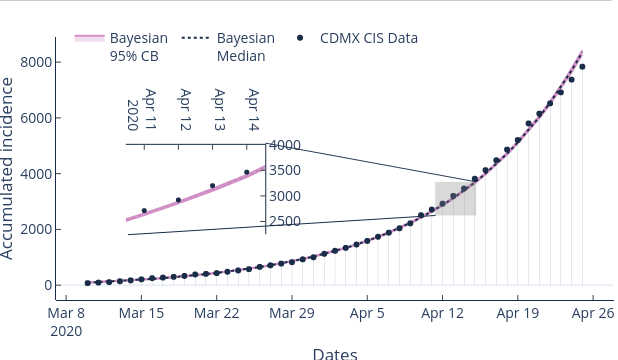
\includegraphics[width=0.8\textwidth, keepaspectratio]{%
			assets/MCMC_CDMXDataFitting.png%
		}
		\caption{%
			MCMC Fit of diary new cases of Mexico city
			during exponential growth. See
			\url{https://plotly.com/~sauld/53/} for an electronic
			version.
		}
		\label{fig:data_CDMX_fitting}
	\end{figure}
\end{frame}

